{\color{teal!90}\chapter{User Interface}\label{cap:ui}}

\AddToShipoutPictureBG*{%
  \AtPageUpperLeft{%
    \raisebox{-\height}{%
      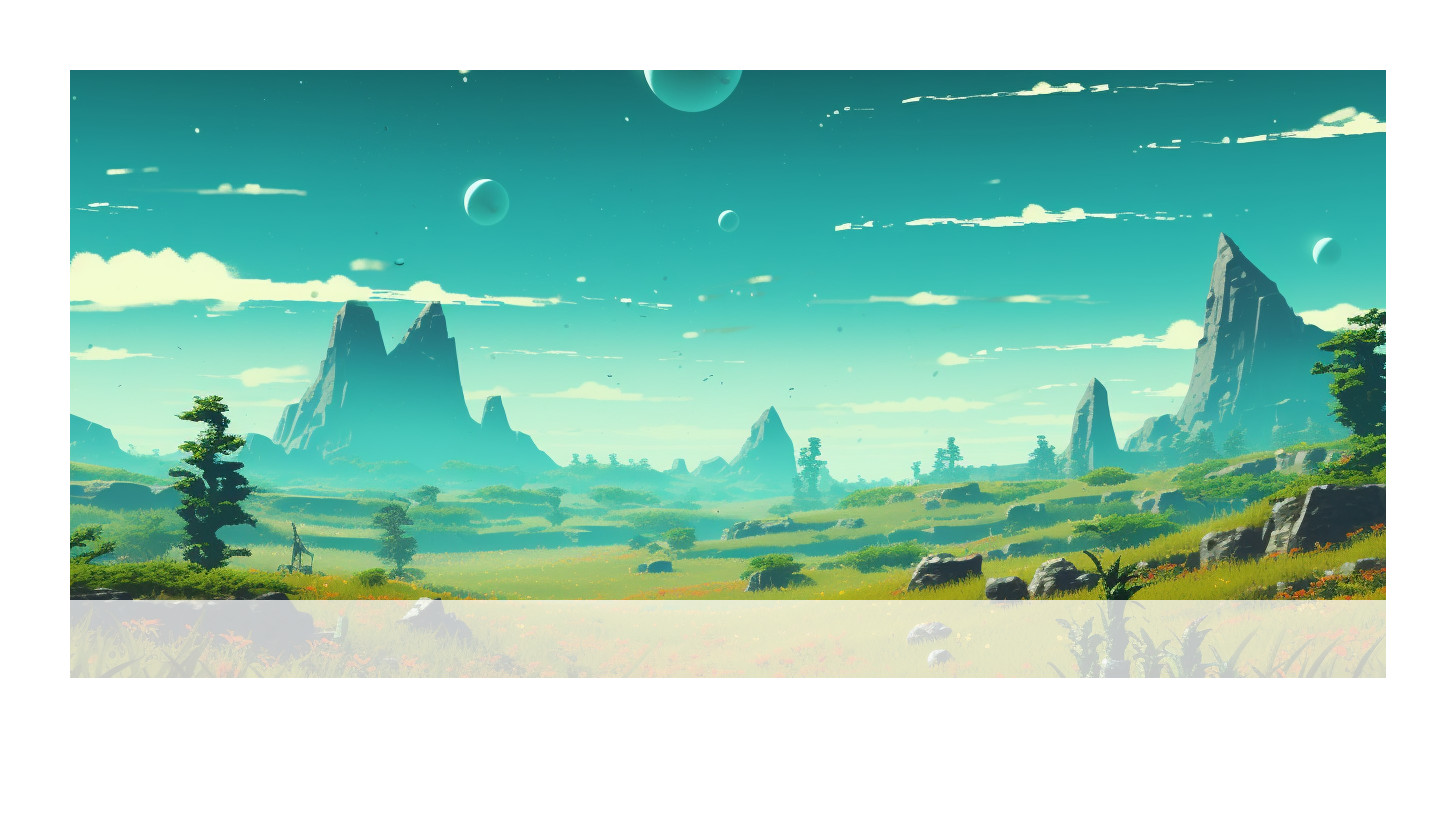
\includegraphics[width=\paperwidth]{./chapters/user-interface.jpg}%
    }%
  }
}

\minitoc% Creating an actual minitoc mini lista contenuti


\section{The Look}

\simplewrap{13}{R}{8cm}{8cm}{./chapters/user-interface/ui-clock.png}{-10pt}{Temporary Prototype of the \gls{ui} showing clock and console}{fig:clock}

On September 7\textsuperscript{th}, after re-enabling \gls{navisettings}, which serves as the system app for navigation and other functions, I made some notable visual adjustments (fig. \ref{fig:clock}):

\begin{enumerate}
    \item I relocated the console (which will eventually transform into a widget) to the side of the app's interface. This change allows for a cleaner main view and opens up more space for other essential features.
    
    \item I introduced a dedicated view to display the current time, with updates occurring every 1000 milliseconds (1 second). This time-display functionality is managed by a class named \texttt{TimeUpdater}. Notably, this class was integrated using Dagger2 for dependency injection, eliminating the need for direct \texttt{findViewById(R.id.timeTextView)} usage in \texttt{MainActivity.kt}.
\end{enumerate}

These alterations contribute to an improved app appearance and functionality. The console's new side placement offers convenience, and the real-time clock display, powered by \texttt{TimeUpdater} and managed through Dagger2, enhances the user experience.

\clearpage
\subsection{2023-09-08 update}
\simplewrap{13}{R}{8cm}{8cm}{./chapters/user-interface/ui-central-clock.jpg}{-10pt}{Improved resolution of the \gls{ui} showing clock at the center}{fig:central-clock}

I have made some more changes to the UI, as shown in figure \ref{fig:central-clock}. The clock is now at the center of the screen, and the console is on the right side. I have also added a background image, which is the same as the system wallpaper. This is a temporary solution to the wallpaper issue, which I will address later in this chapter.

\medskip
Also the clock is now updating every minute, instead of every second. This still didn't resolve the lag issue. I will need to investigate further.

\clearpage
\section{settingsButtonClickListener}
The injection shown in Listing \ref{lst:weird-injection} keeps the MainActivity cleaner, but it may seem unconventional as the injected object is never directly used. It returns a listener, which, in this case, isn't utilized since all the initialization is done during build time. Is this the right approach? While it serves its purpose, one might question if it aligns with best practices.
\lstinputlisting[language=Kotlin,linewidth=0.8\linewidth,caption={Weird Injection}, label=lst:weird-injection, escapechar=\%]{./chapters/code/weird-injection.kt}

\section{Wallpaper}
Even though this app is now the default launcher, the wallpaper displayed on boot differs from what's expected. To temporarily address this issue, I have applied a single image as both the system wallpaper and the app layout background. However, there is significant work ahead in translating the Java code from the CTOUCH project to Kotlin for the Taishan project. This includes implementing policies using SharedPreferences to allow users to change the wallpaper and make it permanent once selected. Currently, this is just for a quick look, as other more pressing matters demand my attention. Therefore, I'll tackle this aspect towards the end of the project.

\subsection{Wallpaper Resolution}
I did upscale the image to 5824x3264, which is higher than Taishan's resolution. This is to ensure that the image is not stretched or distorted when displayed on the screen. However, this is not the optimal solution, as it increases the app's size. I will need to find a way to downscale the image to the correct resolution without compromising the image quality.
Maybe even performances could be affected by this, but I will need to test this hypothesis. Or maybe it's the clock updating every second that is causing the lag.

\section{The DebugConsole}
The DebugConsole is now a widget that can be moved around the screen. It can't be resized yet, but it can be moved around. It disappears and appears on demand by clicking the \texttt{Shell Button}\footnote{The Shell Button is handled with \textbf{ConsoleToggleButtonClickListener} which is injected in the MainActivity.kt using Dagger2.}.

\section{The Recycler View}
The Recycler View is now working. It displays a list of all the features that are currently implemented. Injections are also working, and the code is cleaner.

\section{Features Implemented}
\begin{itemize}
    \item \textbf{Clock} - The clock is now at the center of the screen. It updates every minute. It is powered by \textbf{TimeUpdater} and managed through \gls{dagger2}.
    \item \textbf{DebugConsole} - The DebugConsole is now a widget that can be moved around the screen. It can't be resized yet, but it can be moved around. It disappears and appears on demand by clicking the \texttt{Shell Button}. It is managed through \gls{dagger2}.
    \item \textbf{App Drawer} - The App Drawer is now a Recycler View that displays a list of all the apps that are currently installed on the device. It is powered by \textbf{AppListAdapter} and managed through \gls{dagger2}.
    \begin{enumerate}
        \item \textbf{Launch it via Remote Control} - The App Drawer can be launched via the Remote Control by pressing the \faWindows\ button.
    \end{enumerate}
\end{itemize}